\chapter{A research cycle, end to end}\label{ch:cycle}

\noindent\emph{Nothing in this book is investment advice. Every
number is a lesson, not a recommendation.}

\medskip
\noindent Every earlier chapter answered one question well:
returns, microstructure, backtests, validation, sizing. This
chapter walks the whole loop once on the book's own pinned tape,
in the order a desk actually runs it --- and it starts with a
confession. Midway through writing this book, the pinned
\texttt{btc\_daily.csv} turned out to be \emph{scrambled}: its
\texttt{c} column was not close at all, but VWAP. A quarter of
the book's quoted statistics were computed on the wrong column.
The bug was caught, the file refetched and corrected, and every
downstream number re-verified --- and the autopsy itself is the
cleanest possible first lesson for this chapter: \emph{the data
contract comes before the hypothesis}.

\begin{figure}[htbp]\centering
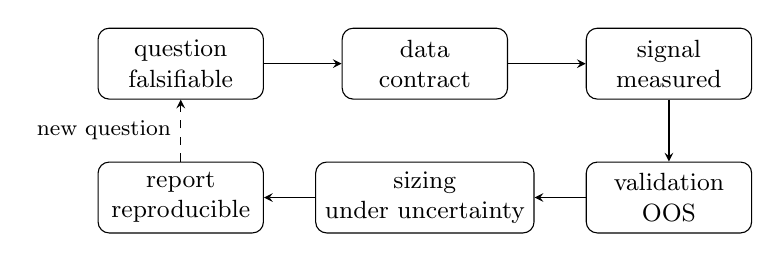
\begin{tikzpicture}[font=\small, >=stealth,
  box/.style={draw, rounded corners, align=center, minimum width=2.1cm, minimum height=0.9cm}]
\node[box] (q)  at (0,0)      {question\\falsifiable};
\node[box] (d)  at (3.1,0)    {data\\contract};
\node[box] (s)  at (6.2,0)    {signal\\measured};
\node[box] (v)  at (6.2,-1.7) {validation\\OOS};
\node[box] (sz) at (3.1,-1.7) {sizing\\under uncertainty};
\node[box] (rp) at (0,-1.7)   {report\\reproducible};
\draw[->] (q) -- (d); \draw[->] (d) -- (s); \draw[->] (s) -- (v);
\draw[->] (v) -- (sz); \draw[->] (sz) -- (rp);
\draw[->, dashed] (rp) -- (q) node[midway,left,font=\footnotesize]{new question};
\end{tikzpicture}

\caption{The cycle this chapter walks once, end to end. Every
arrow is a place where honesty can leak: the data-contract step
is the one this book almost skipped --- and the one this chapter
opens with.}
\label{fig:cycle}
\end{figure}

\section{The question: falsifiable or nothing}\label{sec:question}

``Is momentum real?'' is not a research question --- it has no
stopping condition. A falsifiable question names the horizon,
the instrument, and the verdict that would kill it. Ours:
\emph{on the pinned BTC daily tape, does a 20-day momentum rule
earn a positive risk-adjusted return out of sample?} Three ways
this dies: the edge is not distinguishable from zero; it
disappears out of sample; or the file it was measured on turns
out to lie. As it happens, we get to watch all three.

\begin{example}\label{ex:falsifiable}
\textbf{Write the kill conditions first.} Before touching data,
fix the three statements that would end the investigation:
(i)~the measured mean is within $2\sigma$ of zero; (ii)~the
out-of-sample half does not confirm the in-sample half;
(iii)~the dataset fails its contract checks. Any one of them
kills the strategy --- and as we will see, all three fire.
\begin{solution}
The discipline is ordering: kill conditions written \emph{before}
the measurement cannot be renegotiated afterwards. This is the
statistical version of writing unit tests before the code --- and
the reason ch09's multiple-testing chapter exists.
\end{solution}
\end{example}

\section{The data contract}\label{sec:contract}

A pinned file is a \emph{claim}, and claims get audited. The
contract for an OHLC daily bar file is mechanical: the open of a
continuous daily series equals the previous close (venues roll
bars at a fixed timestamp, so gaps are cents, not thousands);
the high bounds open and close from above; the low bounds them
from below. Three arithmetic checks, no model, no judgment.

\begin{example}\label{ex:autopsy}
\textbf{Autopsy of a scrambled file.}
\texttt{data\_autopsy.py} runs the three contract checks on
both the file that was shipped --- \texttt{btc\_daily\_scrambled.csv}
--- and the corrected refetch, \texttt{btc\_daily.csv}:
\begin{verbatim}
btc_daily_scrambled.csv: header=['time', 'o', 'h', 'l', 'c']
  max |open_t - close_{t-1}| =     10115.10  (real daily bars: ~0)
  'high' col violations h>=o,h>=c: 721
  'low'  col violations l<=o,l<=c: 384
btc_daily.csv: header=['time', 'o', 'h', 'l', 'c']
  max |open_t - close_{t-1}| =        62.90  (real daily bars: ~0)
  'high' col violations h>=o,h>=c: 0
  'low'  col violations l<=o,l<=c: 0
  col2>=all? True
\end{verbatim}
The original file fails all three checks on nearly every row:
its ``open'' sat \$10{,}115 from the previous close, and what it
called \texttt{h} was below both putative open and close on
\emph{all 721 rows} --- impossible for a real high. Reading the
columns against live Kraken data resolved it: the file's columns
were (time, high, low, close, vwap) under an
\texttt{o,h,l,c} header. The VWAP had been quietly playing the
role of close in every downstream statistic.
\begin{solution}
The diagnosis ran in one afternoon because the contract was
mechanical: no model of ``what prices should look like,'' just
order relations the file could not satisfy. A data contract is
executable documentation --- \texttt{pin\_data.py} (ch07) records
the sha256; \texttt{data\_autopsy.py} records \emph{what the
columns must mean}.
\end{solution}
\end{example}

\begin{figure}[htbp]\centering
\begin{tikzpicture}
\begin{axis}[width=0.82\linewidth, height=5cm, ybar, bar width=10pt,
  ymin=0, symbolic x coords={hgap,hviol,lviol}, xtick=data,
  xticklabels={max $|o_t-c_{t-1}|$, $h$-violations, $l$-violations},
  ylabel={count / dollars}, legend style={at={(0.5,1.02)},anchor=south,legend columns=-1,font=\small},
  nodes near coords, every node near coord/.append style={font=\tiny}]
\addplot table[x index=0,y=scram] {figures/data/ch17-autopsy.dat};
\addplot table[x index=0,y=corr] {figures/data/ch17-autopsy.dat};
\legend{scrambled file, corrected file}
\end{axis}
\end{tikzpicture}

\caption{Three mechanical checks expose the scrambled file: the
putative open was \$10{,}115 away from the previous close
(left), the column marked \texttt{h} failed $h\ge\max(o,c)$ on
all 721 rows, and the column marked \texttt{l} failed
$l\le\min(o,c)$ on 384. The corrected file fails none.}
\label{fig:autopsy}
\end{figure}

\begin{example}\label{ex:manufactured}
\textbf{The defect was not benign --- it manufactured a signal.}
VWAP is an intraday volume-weighted average; averaging smooths
the series, and smoothing invents autocorrelation. On the
scrambled file the 20-day momentum rule showed a tempting
Sharpe $+0.70$. On the corrected file: $+0.26$. The ``edge''
was a property of the column mix-up, not of the market.
\begin{solution}
\texttt{signal\_scan.py} run on each file prints the same
convention applied to both (Figure~\ref{fig:signal}). This is
the second-order lesson: a data bug does not merely add noise
to your statistics --- it can \emph{create structure} that looks
like an edge. Kurtosis read $+2.01$ instead of $+4.56$ on the
scrambled file; lag-1 return autocorrelation read $+0.281$
instead of $-0.031$. Both errors were the same mechanism:
averaging pulls a series toward smoothness, so fat tails thin
out and neighbouring returns start to agree.
\end{solution}
\end{example}

\begin{figure}[htbp]\centering
\begin{tikzpicture}
\begin{axis}[width=0.72\linewidth, height=5cm, ybar, bar width=12pt,
  symbolic x coords={mom1,mom20}, xtick=data, ymin=-0.2, ymax=1.0,
  ylabel={annualised Sharpe}, legend style={at={(0.5,1.02)},anchor=south,legend columns=-1,font=\small},
  nodes near coords, every node near coord/.append style={font=\tiny}]
\addplot table[x index=0,y=scram] {figures/data/ch17-signal.dat};
\addplot table[x index=0,y=corr] {figures/data/ch17-signal.dat};
\legend{on scrambled file, on corrected file}
\end{axis}
\end{tikzpicture}

\caption{Twenty-day momentum reads Sharpe $+0.70$ on the
scrambled file and $+0.26$ on the corrected one; one-day
momentum goes from $-0.03$ to $+0.18$. The defect did not just
shift numbers --- it invented a strategy.}
\label{fig:signal}
\end{figure}

\section{The signal, measured honestly}\label{sec:signal}

With a corrected file and a fixed convention --- position on
day~$i$ uses only the signal $c_{i-1}/c_{i-1-L}-1>0$ ---
\texttt{signal\_scan.py} measures both candidates:
\begin{verbatim}
file: btc_daily.csv
mom1: n=357  mean_when_long=+2.16bp/day  ann_sharpe=+0.18
mom20: n=350  mean_when_long=+2.78bp/day  ann_sharpe=+0.26
honest verdict: tiny edge, not the number the other file promised
\end{verbatim}

\begin{example}\label{ex:signal17}
\textbf{Positive is not significant.} The mom20 rule earns
$+2.78$bp on its 350 long days --- nonzero, and useless to
quote alone. The standard error on that mean is $10.78$bp/day:
the estimate is $0.26$ standard errors from zero.
\begin{solution}
This is ch12's Sharpe-CI lesson applied at the source: with
$\hat\mu/\mathrm{SE}\approx 0.26$, the data are equally
compatible with a small positive edge and with none at all. The
honest sentence is not ``momentum works'' or ``momentum fails''
--- it is ``this tape cannot distinguish them.''
\end{solution}
\end{example}

\section{Validation: the split-sample}\label{sec:validate}

The cheapest OOS test is chronological: do the first half's
long days and the second half's agree?

\begin{example}\label{ex:wf17}
\textbf{The edge halves, then vanishes.}
\texttt{cycle\_walkforward.py} splits the mom20 long-day
returns:
\begin{verbatim}
IS half : n=175  sharpe +0.54  mean +5.55bp
OOS half: n=175  sharpe +0.00  mean +0.01bp
full    : ret +10.2%  sharpe +0.26
\end{verbatim}
First half $+5.55$bp, second half $+0.01$bp: whatever the rule
found, it was in the early tape and it did not repeat. The
full-sample $+0.26$ Sharpe is the average of a real half and an
empty one.
\begin{solution}
Compare ch11's anchored-walk-forward decay: edges that live in
one regime do not transfer. And note the trap we avoided: on the
\emph{scrambled} file the candidate looked twice as strong,
which is exactly how a bad dataset produces a confident paper.
\end{solution}
\end{example}

\begin{figure}[htbp]\centering
\begin{tikzpicture}
\begin{axis}[width=0.6\linewidth, height=4.5cm, ybar, bar width=18pt,
  symbolic x coords={IS,OOS}, xtick=data, ymin=0, ymax=0.8,
  ylabel={annualised Sharpe}, nodes near coords, every node near coord/.append style={font=\small}]
\addplot table[x index=0,y=sharpe] {figures/data/ch17-wf.dat};
\end{axis}
\end{tikzpicture}

\caption{Split-sample honesty on the corrected tape: $+0.54$ in
the first half of the long days, $+0.00$ in the second.}
\label{fig:wf17}
\end{figure}

\begin{figure}[htbp]\centering
\begin{tikzpicture}
\begin{axis}[width=0.82\linewidth, height=5cm, xlabel={bar}, ylabel={equity},
  legend style={at={(0.02,0.98)},anchor=north west,font=\small}, ymin=0.8]
\addplot[blue!60!black, thick] table[x index=0,y index=1] {figures/data/ch17-equity-corr.dat};
\addplot[gray, dashed] table[x index=0,y index=2] {figures/data/ch17-equity-corr.dat};
\legend{mom20 strategy (corrected data), buy \& hold}
\end{axis}
\end{tikzpicture}

\caption{The honest equity curve: the mom20 rule ends $+10.2\%$
against buy-and-hold's $+24.0\%$ --- positive, real, and worse
than doing nothing.}
\label{fig:eq17}
\end{figure}

\section{Sizing under uncertainty}\label{sec:size17}

Even taken at face value, what would the measured edge justify?
Continuous-Kelly on the long days:

\begin{verbatim}
when long: mean +2.78bp/day  se 10.78bp  var 4.07e-04
continuous-Kelly f* = +0.68
mu is +0.26 SEs from zero -- inside the noise band,
so the honest position is: f* = 0.  There is nothing to size.
\end{verbatim}

\begin{example}\label{ex:kelly17}
\textbf{$f^*$ is a function of a number you do not have.}
Figure~\ref{fig:kelly17} draws $\hat f^*=\hat\mu/\hat\sigma^2$
against the assumed mean. At the point estimate, $f^*=0.68$;
across the $95\%$ band on $\hat\mu$ it runs from $-4.51$ to
$+5.87$ --- through zero.
\begin{solution}
ch13's estimation-error table, one level deeper: when the
confidence interval on the edge contains zero, the confidence
interval on the optimal bet contains zero, and the sizing
decision is dominated by the estimation error, not the edge.
A nominal $f^*>0$ computed on an insignificant mean is not a
position --- it is a rounding artefact with a leverage dial.
\end{solution}
\end{example}

\begin{figure}[htbp]\centering
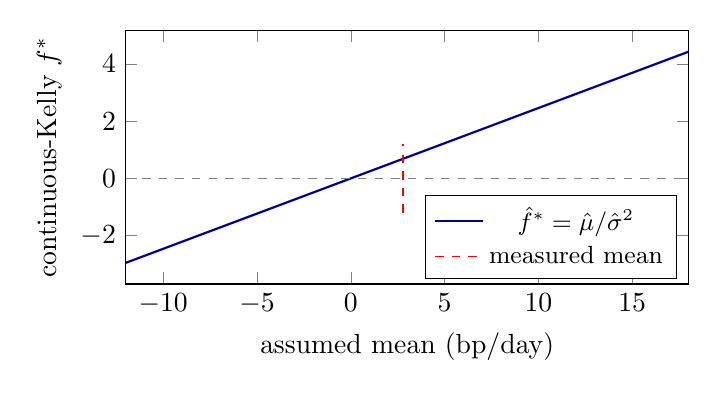
\begin{tikzpicture}
\begin{axis}[width=0.72\linewidth, height=4.8cm, xlabel={assumed mean (bp/day)},
  ylabel={continuous-Kelly $f^*$}, xmin=-12, xmax=18,
  legend style={at={(0.98,0.02)},anchor=south east,font=\small}]
\addplot[blue!60!black, thick, domain=-12:18, samples=60] {x*1e-4/4.07e-4};
\addplot[red, dashed] coordinates {(2.78,-1.2) (2.78,1.2)};
\addplot[gray, dashed, domain=-12:18] {0};
\legend{$\hat f^*=\hat\mu/\hat\sigma^2$, measured mean}
\end{axis}
\end{tikzpicture}

\caption{$\hat f^*$ as a function of the assumed mean. At the
measured $2.78$bp it is $+0.68$; across the uncertainty band it
crosses zero. The defensible answer is $f^*=0$.}
\label{fig:kelly17}
\end{figure}

\section{The report: reproducible or it didn't happen}\label{sec:report}

The deliverable of a research cycle is a memo every number of
which can be regenerated from the pinned file by one command.
\texttt{memo\_render.py} does not quote results --- it
\emph{computes} them:
\begin{verbatim}
MEMO: daily BTC 20-day momentum, pinned tape 2024-10..2026-09
  n=720 daily returns, sd=0.444 ann
  mom20 edge +2.78bp/day when long; split-sample sharpe +0.54 -> +0.00
  claim: REJECTED -- not an edge at daily horizon on this tape
\end{verbatim}

\begin{example}\label{ex:memo17}
\textbf{A rejected claim is a finished project.} The memo's
verdict is \texttt{REJECTED} --- not ``inconclusive,'' not
``promising.'' The kill conditions fired: insignificant mean,
no OOS confirmation, and a data file that had to be repaired
before it could be trusted at all.
\begin{solution}
ch15's checklist applied: one falsifiable claim, measured on a
contract-audited file, validated out of sample, sized under
uncertainty, reported with its regeneration script. The most
valuable output a research cycle can produce is a clean
\emph{no} --- it retires a question instead of haunting a
notebook folder.
\end{solution}
\end{example}

\begin{table}[htbp]\centering\small
\begin{tabular}{lll}
\toprule
stage & output & what kills it\\\midrule
question & falsifiable claim + kill conditions & unfalsifiable phrasing\\
data & contract checks, sha256 pin & scrambled columns pass unaudited\\
signal & mean $\pm$ SE, convention stated & mean without error bars\\
validation & IS vs OOS agreement & first half only\\
sizing & $f^*$ under the CI on $\hat\mu$ & nominal $f^*$ on noise\\
report & memo regenerable by one command & prose quoting stale output\\
\bottomrule
\end{tabular}
\caption{The cycle as a checklist. Every row is a gate; the
order matters --- a later stage cannot rescue an earlier lie.}
\end{table}

\section{Common mistakes}
\begin{itemize}
\item \textbf{Auditing the data after the backtest.} The
contract checks cost minutes; the scrambled file cost a
book-wide re-verification. Audit first.
\item \textbf{Treating ``positive mean'' as an answer.} Mean
without standard error is a number, not a result.
\item \textbf{Trusting a single split.} One IS/OOS cut is the
minimum, not the standard --- ch11's walk-forward is the
stronger tool when the question survives this far.
\item \textbf{Sizing on the point estimate.} $\hat f^*$ has a
distribution; its width, not its centre, decides the trade.
\item \textbf{Softening the verdict.} ``Mixed evidence'' on a
dead hypothesis is how dead strategies get traded.
\item \textbf{Prose memos.} If a number in the report is not
produced by running a script, it will drift. The memo is code.
\item \textbf{Assuming data errors add noise.} They add
\emph{structure}: VWAP-as-close invented a +0.70-Sharpe
strategy out of thin air.
\end{itemize}

\section*{Notes}
This chapter is deliberately autobiographical: the scrambled
file is real, the autopsy scripts run, and the rejected claim is
the honest output of the cycle. A reader who reproduces it owns
the full loop --- question, contract, signal, validation,
sizing, report --- which is the actual job this book teaches.

\section*{Further reading}
\begin{itemize}
\item M.~Lopez de Prado, \emph{Advances in Financial Machine
Learning} --- the research-process bible behind ch09 and ch11
(borrow or library).
\item E.~Chan, \emph{Quantitative Trading} and
\emph{Algorithmic Trading} --- the practitioner version of this
cycle (borrow or library).
\item J.~Ottaviani \& P.~Strachan --- academic literature on
momentum's fragility across assets:

\url{https://en.wikipedia.org/wiki/Momentum_investing}
\item Kelly sizing under estimation error (MacLean--Thorp--Ziemba
family):

\url{https://en.wikipedia.org/wiki/Kelly_criterion}
\item The book's own chain: ch07 (pinning), ch08 (harness),
ch11 (walk-forward), ch13 (Kelly), ch15 (reporting).
\end{itemize}

\begin{rulebox}[Watch instead]
\begin{itemize}
\item ``Dangers of Backtest Overfitting'' --- Marcos Lopez de
Prado, Alex Bernal channel (20:41). Why research processes
fail at the validation step; opened and verified 2026-10-11.
\url{https://www.youtube.com/watch?v=QxhxLwNbMMg}
\item ``How quant trading strategies are developed and tested
w/ Ernie Chan'' --- Chat With Traders (60:38). A working
researcher's version of this chapter's cycle; opened and
verified 2026-10-11.
\url{https://www.youtube.com/watch?v=DW9zQ8Hz6gQ}
\end{itemize}
\end{rulebox}

\section*{Exercises}
\subsection*{Easy}
\begin{enumerate}
\item Write the three-order-relation contract for an OHLC file
in your own words, and state which of the three the scrambled
file violated most severely. (Answer: $h\ge\max(o,c)$ failed
on all 721 rows.)
\item \texttt{data\_autopsy.py} reports
\texttt{max |open\_t - close\_\{t-1\}| = 62.90} on the
corrected file --- not zero. Why can a real daily open differ
from the previous close by \$62.90? (Answer: bar boundaries are
exchange timestamps; trades around the boundary print at
different prices, and a quiet overnight tape can leave a small
true gap.)
\item The scrambled file's \texttt{c} was VWAP. Give the
one-sentence mechanism for why that lowered measured excess
kurtosis ($+4.56\to+2.01$). (Answer: intraday averaging pulls
each day's ``close'' toward the day's mean, shrinking extreme
daily moves.)
\item What does \texttt{pin\_data.py}'s sha256 prove, and what
does it \emph{not} prove? (Answer: proves the bytes are
unchanged since pinning --- proves nothing about whether the
columns mean what the header claims.)
\item Why does \texttt{signal\_scan.py} take the file path as an
argument? (Answer: so the identical convention measures both
files --- the comparison is apples-to-apples.)
\end{enumerate}
\subsection*{Medium}
\begin{enumerate}
\item Reproduce the autopsy on \texttt{btc\_trades.csv}:
write its contract checks (price $>0$, size $>0$, timestamps
non-decreasing) and run them.
\item The memo claims \texttt{REJECTED}. Rewrite it as
\texttt{INCONCLUSIVE} and defend which verdict the evidence
actually supports --- what would change your answer?
\item On the corrected file, run \texttt{signal\_scan.py}'s
convention for $L\in\{5,10,60\}$. Does any horizon look
significant after the SE correction? State the honest verdict.
\item Show why averaging invents autocorrelation: let
$\tilde r_t=(r_t+r_{t-1})/2$ and compute
$\operatorname{corr}(\tilde r_t,\tilde r_{t-1})$ when $r$ is
iid. (Answer: $+0.5$ --- half of today's smoothed return is
yesterday's.)
\item \texttt{data\_autopsy.py}'s \texttt{lviol} count is 384,
not 721. What column assignment makes exactly that many rows
violate $l\le\min(o,c)$? Explain.
\end{enumerate}
\subsection*{Hard}
\begin{enumerate}
\item The scrambled file produced a $+0.70$-Sharpe mom20
strategy. Estimate how much of that Sharpe the VWAP smoothing
\emph{must} add mechanically (use the iid-smoothing argument of
Exercise 12), and discuss whether the residual could still be
real momentum.
\item Design the data contract for a tick-level LOB file:
which order relations must hold between bid, ask, trade price,
and timestamps? Which are contract violations vs. merely
suspicious?
\item A teammate proposes fixing the defect by
``just re-deriving the statistics on the corrected file.''
What does the pipeline additionally require before the book is
honest again? (Hint: tests, figures, and prose all carry
numbers.)
\end{enumerate}
